\documentclass[PMO,lsstdraft,authoryear,toc]{lsstdoc}
% lsstdoc documentation: https://lsst-texmf.lsst.io/lsstdoc.html
%\input{meta}%

% Package imports go here.
\usepackage{caption}
\usepackage{subcaption}
\usepackage{fancyhdr}
\usepackage{parcolumns} % <<<<<<----- Required
\usepackage{lipsum} % <<<<---- Only needed in the example
\usepackage{hyperref}
% Local commands go here.

%If you want glossaries
%\input{aglossary.tex}
%\makeglossaries

\title{Summit Onboarding Procedure}

% Optional subtitle
% \setDocSubtitle{A subtitle}

\author{%
Diego Tapia, Cristian Silva
}

\setDocRef{ITTN-045}
\setDocUpstreamLocation{\url{https://github.com/lsst-it/ittn-045}}

%\date{\vcsDate}%   <
\date {\today}
% Optional: name of the document's curator
% \setDocCurator{The Curator of this Document}

\setDocAbstract{%
 This ITTN was created to document the procedure of requesting access to the various services located at the summit.
 
}

\setDocChangeRecord{%
  \addtohist{1}{2021-04-12}{Unreleased.}{Cristian Silva}
  \addtohist{2}{2021-05-01}{First Draft}{Diego Tapia}
  \addtohist{3}{2021-05-27}{Second Draft}{Cristian Silva}
  \addtohist{4}{2021-05-31}{Third Draft}{Diego Tapia}
}


\begin{document}

% Create the title page.
\maketitle
% Frequently for a technote we do not want a title page  uncomment this to remove the title page and changelog.
% use \mkshorttitle to remove the extra pages
\section{Introduction}

The access to servers and services of the summit are managed by several backends.

The access to servers (ssh) and VPN is controlled by the IPA backend. To request an IPA account please refer to the section \hyperref[sec:IPA]{Requesting an IPA Account}

The acccess to Nublado is controlled by a Github backend. To request Nublado access please refer to \hyperref[sec:Nublado]{Requesting Nublado Access}.

The access to Wifi is controlled by domain credentials. To request Domain Credentials please refert to \hyperref[sec:Domain]{Requesting Domain Credentials}.
\newpage

\section{How to request an IPA Account / VPN Access for Cerro Pachon Services}

\subsection{IHS Ticket Creation}
  
  To request an IPA account, it is required for the user to create a Service Request ticket inside the IT User Support Dashboard.
  Please check the example below.

\subsubsection{Example}

  Head over to https://jira.lsstcorp.org and log in with your domain account credentials.

\begin{figure}
  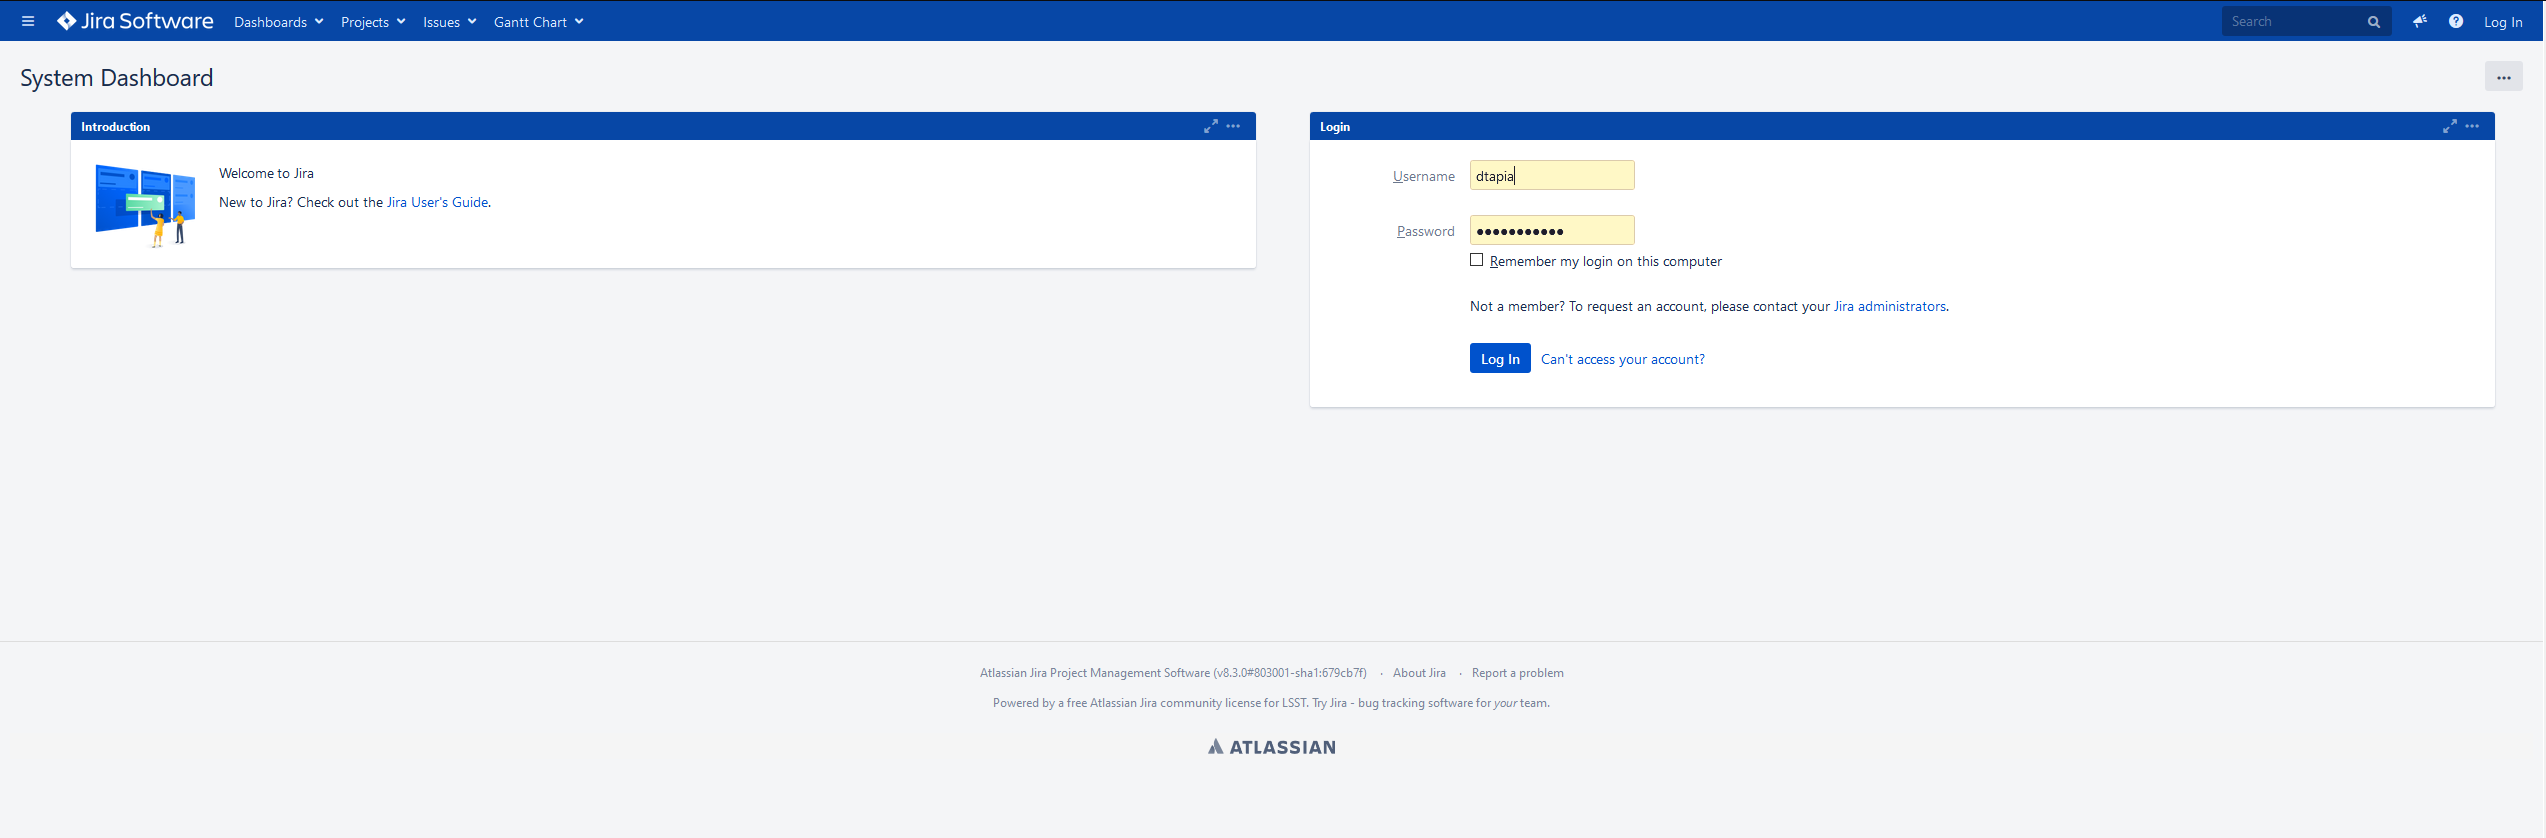
\includegraphics[width=15cm]{Images/example1.png}
  \centering
\end{figure}

\newpage

Once logged in the user will be prompted with the following windows if not similar. Before creating the ticket,  it is required for the user to check that he is in the proper dashboard for this particular case the IT Support Das

\begin{figure}
  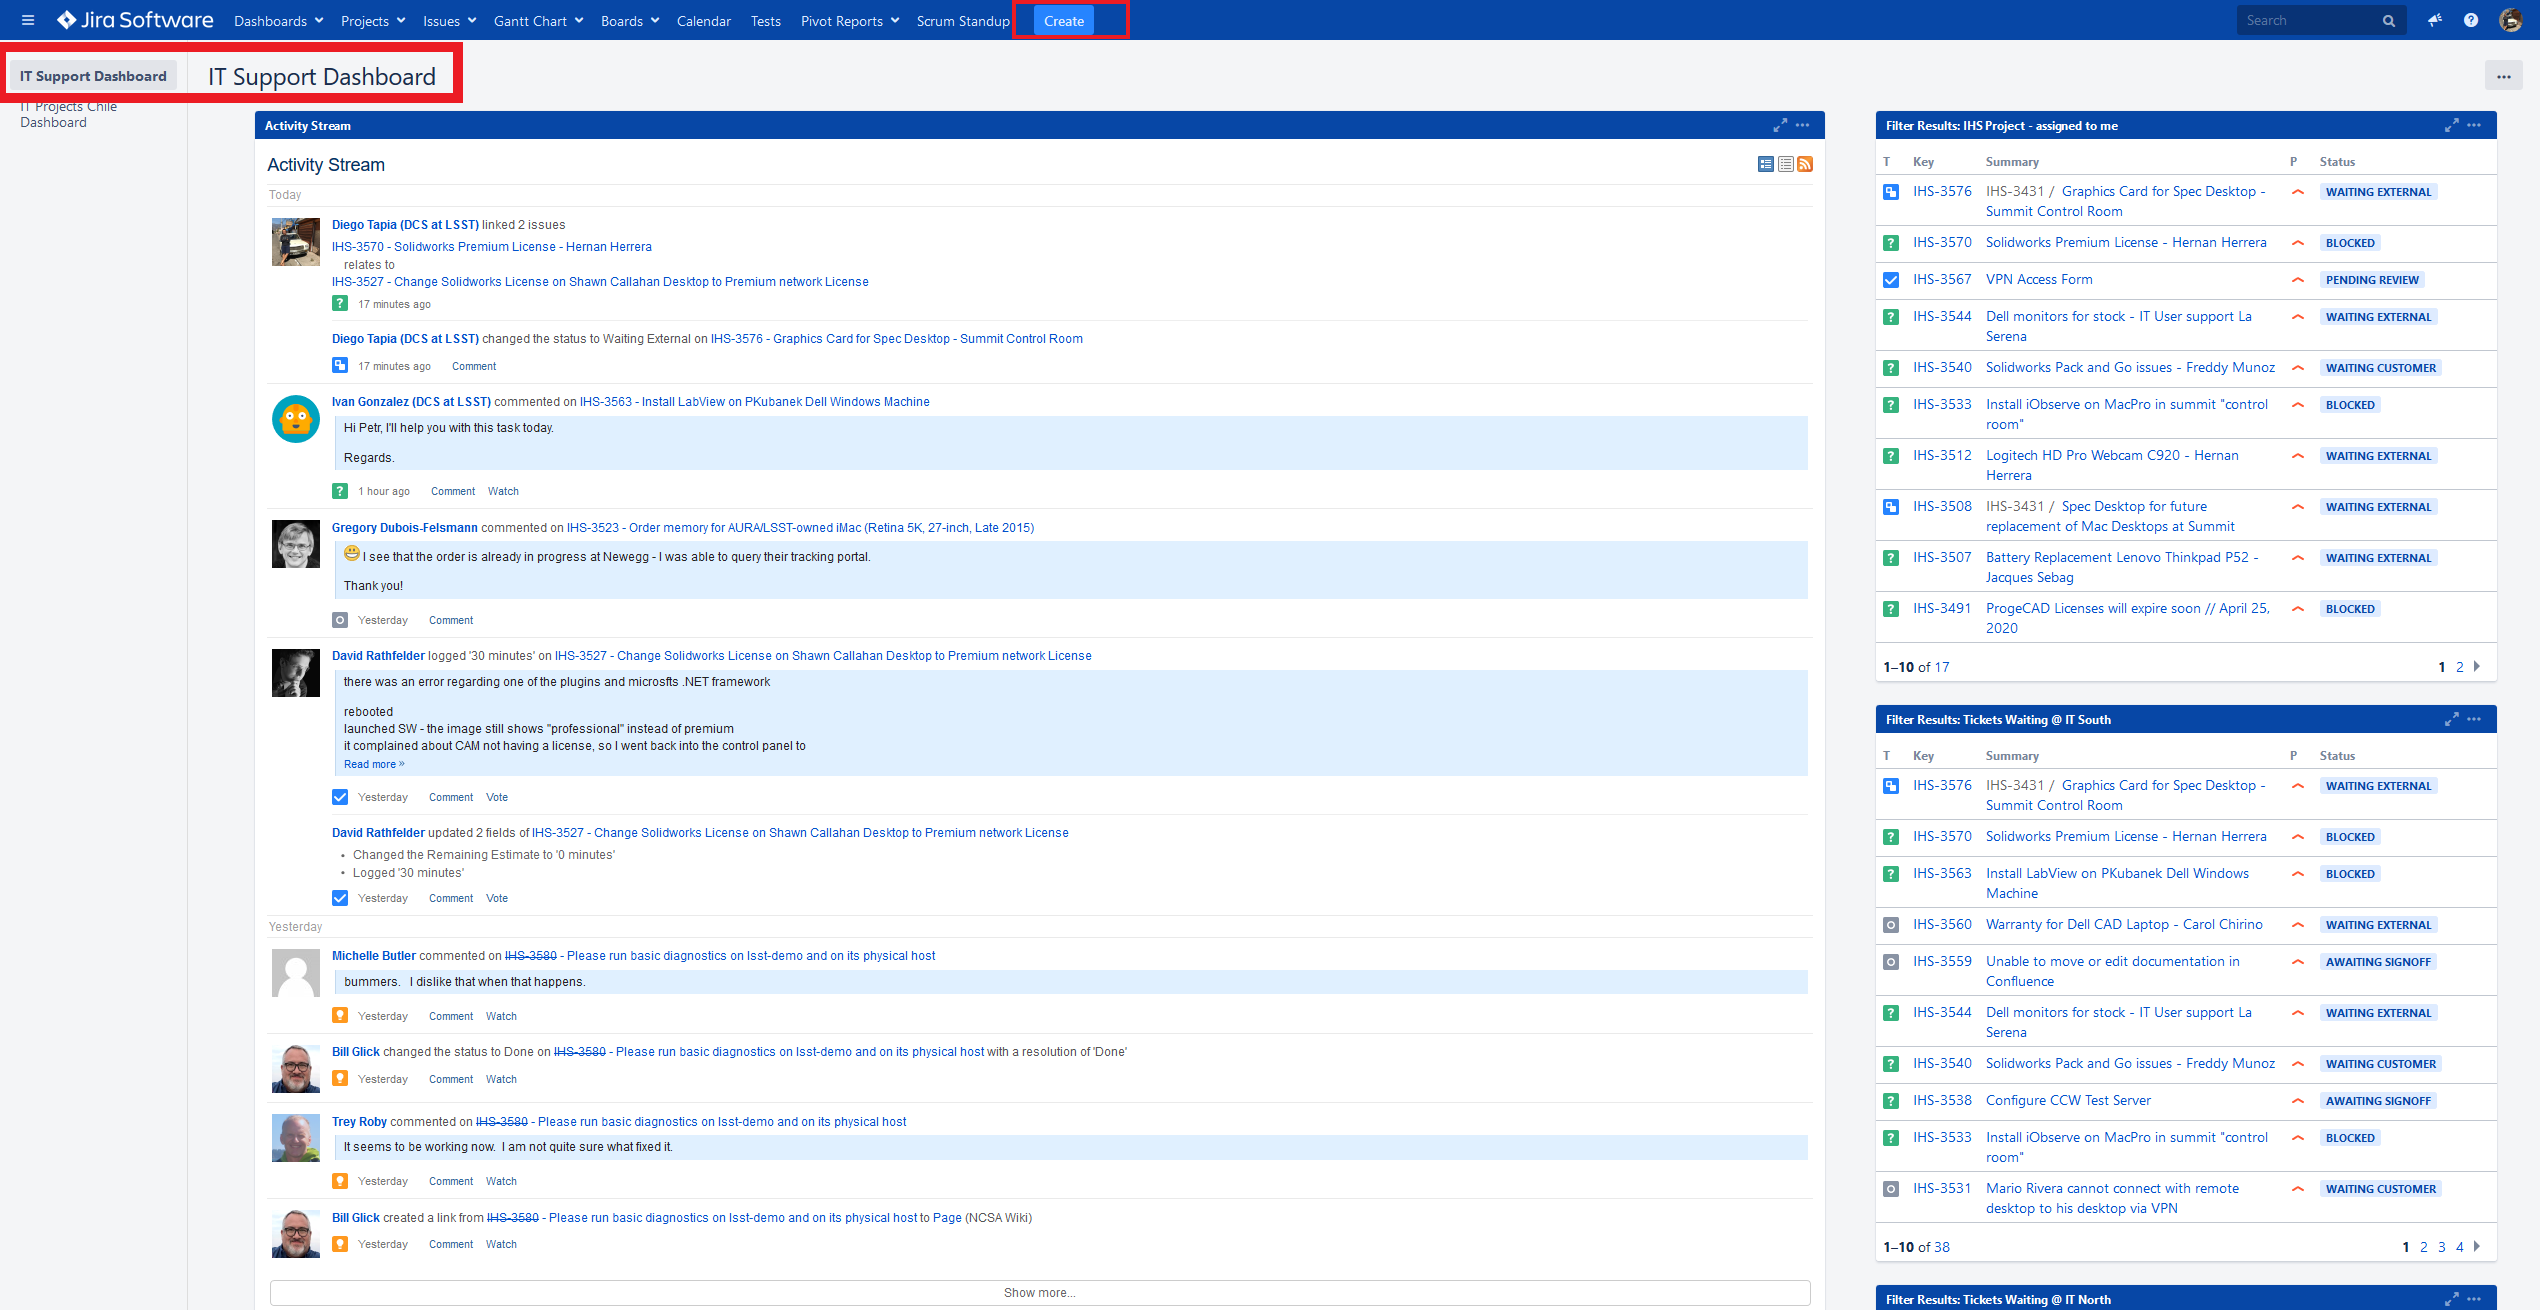
\includegraphics[width=15cm]{Images/example2.png}
  \centering
\end{figure}

On the ticket creation window fill out the template using the information provided below:

\begin{itemize}
  \item Project: IT Helpdesk Support (IHS)
  \item Issue Type: Service Request
  \item Summary: IPA Account Creation / VPN Access - "Insert your name here"
  \item Component: AAA
  \item Description: Copy and Paster the following information and fill out the form.
\end{itemize}

\begin{itemize}
  \item First Name and Last Name: (.......)
  \item Please attach an SSH Public Key: (.......)
  \item Please indicate a valid email address: (.......)
  \item Please state the level of access required or hosts you wish to connect to: (.......)
\end{itemize}

Once all the information is filled out, select the Create option located at the bottom to create the ticket inside IHS IT Support Dashboard.

\begin{figure}
  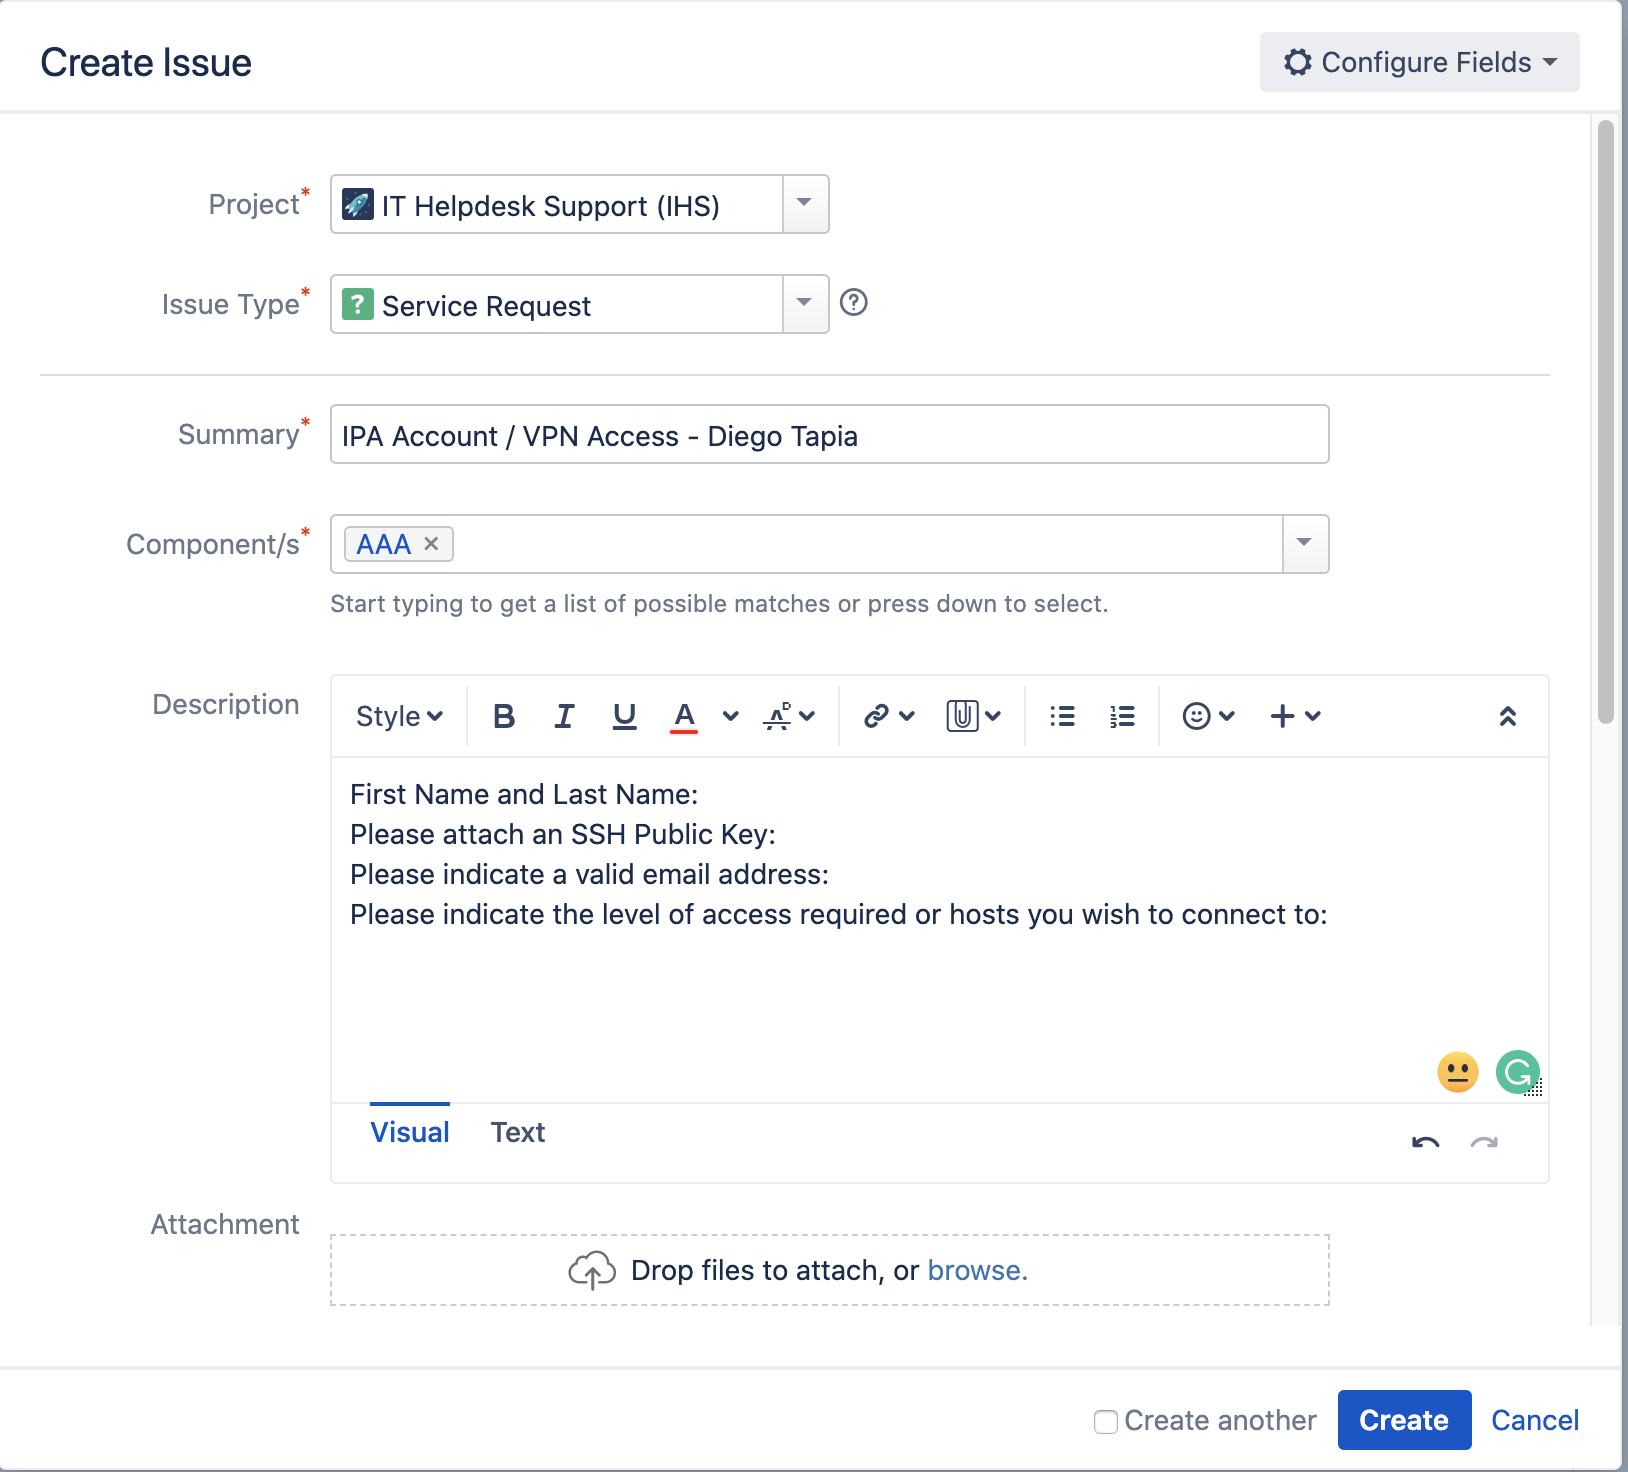
\includegraphics[width=15cm]{Images/example3.png}
  \centering
\end{figure}

IT User support will receive the request and will proceed with the account creation process. Once the account has been created and the services have been provisioned IT Support will be in contact with you via email to provide you with the account credentials and services you've been granted access too along with the website where you can change your temporary password.


IF you have any questions or concerns regarding the services provisioned please contact IT User Support at RubinObs-IT- las@lsst.org

% You can also use the \input command to include several content files.

\appendix
% Include all the relevant bib files.
% https://lsst-texmf.lsst.io/lsstdoc.html#bibliographies
%\section{References} \label{sec:bib}
\renewcommand{\refname}{} % Suppress default Bibliography section
\bibliography{local,lsst,lsst-dm,refs_ads,refs,books}

% Make sure lsst-texmf/bin/generateAcronyms.py is in your path
%\section{Acronyms} \label{sec:acronyms}
%\input{acronyms.tex}
% If you want glossary uncomment below -- comment out the two lines above
%\printglossaries

\end{document}
